\documentclass[12pt,letterpaper, onecolumn]{exam}
\usepackage{amsmath}
\usepackage{amssymb}
\usepackage{graphicx}
\usepackage{setspace}
\usepackage{nicefrac}
\usepackage{hyperref}
\setcounter{MaxMatrixCols}{20}
\usepackage[lmargin=71pt, tmargin=1.2in]{geometry}  %For centering solution box
\lhead{Principles of Navigation}
\rhead{Noah Miller}
\thispagestyle{empty}   %For removing header/footer from page 1

\begin{document}

\begingroup
\centering
\LARGE Principles of Navigation\\
\LARGE Homework 2 \\[0.5em]
\large \today\\[0.5em]
\large Noah Miller\par
\large 903949330\par
\large MECH 6970\par
\endgroup
\pointsdroppedatright   %Self-explanatory
\printanswers
\renewcommand{\solution}{\noindent\textbf{Answer:}\enspace}   %Replace "Ans:" with starting keyword in solution box



\begin{questions}
    \question{Pedestrian Navigation System: Use your phone to implement a pedestrian navigation
        system. Estimate your position by starting at a known location and dead reckoning using
        an open-source step counter and compass. Make sure that your route is at least 1 km and
        contains turns in both directions. Use the compass to track your orientation. You can
        record measurements (i.e. step and compass reading) on your phone if you have that
        functionality. Otherwise use pad and paper to track steps and compass changes.

        You may use a default step length (as discussed in class) or try to estimate your step
        length (a priori) using a measuring instrument of your choice (e.g. tape measure or GPS).
        You should update position with each step and orientation at least every time it changes
        significantly. Plot your route on a map background using GPS visualizer
        (\url{https://www.gpsvisualizer.com/}) or a Matlab toolbox if available. Measure the error in
        your final position and orientation. Report total error and error relative to distance
        traveled.}

    \solution{%
        I planned to walk around my apartment complex (Figure \ref{fig:gmap}), totaling $1.5$ kilometers - according to Google Earth. I recorded 22 separate measurements (Table \ref{tbl:1}), noting heading according to the \textit{Compass} app on my iPhone and the number of steps according to the pedometer feature on my Apple Watch SE. Before starting my route, I already walked 4,296 steps that day. Figure \ref{fig:gmap_steps} shows the plotting of my measurements, assuming a constant 1 meter step length. When plotting the trajectory, I assumed the $1\,[cm]:20\,[m]$ scale of the map image to be correct, and drew on top of the image using a ruler/protractor on my iPad mini with my Apple Pencil. My estimated final position compared with my actual final position were off by about 70 meters. The estimated trajectory from Figure \ref{fig:gmap_steps} resembles a similiar shape to my actual path, but shows variations in direction and path lengths as differents points during the route. An assumed constant step length could be a factor in the final error, along with the difficulty of the path. A better route for this problem statement would have distinct left and right turns, instead, this planned route (Figure \ref{fig:gmap}) has curving turns, making it hard to decide when to measure.


        \begin{figure}[!h]
            \centering
            \includegraphics[width=0.5\linewidth]{IMG_0037.PNG}
            \caption{Planned route around apartment complex, using Google Earth to measure.}
            \label{fig:gmap}
        \end{figure}

        \begin{table}[!h]
            \caption{Recorded measurements while walking planned route (Figure \ref{fig:gmap})}
            \label{tbl:1}
            \centering
            \begin{tabular}{|c|c|c|c|c|}
                \hline
                \# & Step Number & Step Difference & Heading [deg] & Heading Difference [deg] \\ \hline
                1  & 4296        & 0               & 176           & 0                        \\
                2  & 4378        & 82              & 159           & -17                      \\
                3  & 4405        & 27              & 238           & 79                       \\
                4  & 4418        & 13              & 240           & 2                        \\
                5  & 4539        & 121             & 266           & 26                       \\
                6  & 4581        & 42              & 321           & 55                       \\
                7  & 4708        & 127             & 356           & 35                       \\
                8  & 4877        & 169             & 5             & -351                     \\
                9  & 4956        & 79              & 65            & 60                       \\
                10 & 5120        & 164             & 178           & 113                      \\
                11 & 5173        & 53              & 273           & 95                       \\
                12 & 5250        & 77              & 161           & -112                     \\
                13 & 5403        & 153             & 120           & -41                      \\
                14 & 5533        & 130             & 177           & 57                       \\
                15 & 5541        & 8               & 260           & 83                       \\
                16 & 5581        & 40              & 210           & -50                      \\
                17 & 5635        & 54              & 171           & -39                      \\
                18 & 5730        & 95              & 120           & -51                      \\
                19 & 5779        & 49              & 68            & -52                      \\
                20 & 5821        & 42              & 340           & 272                      \\
                21 & 5851        & 30              & 57            & -283                     \\
                22 & 5985        & 134             & 45            & -12                      \\ \hline
            \end{tabular}
        \end{table}

        \begin{figure}[!h]
            \centering
            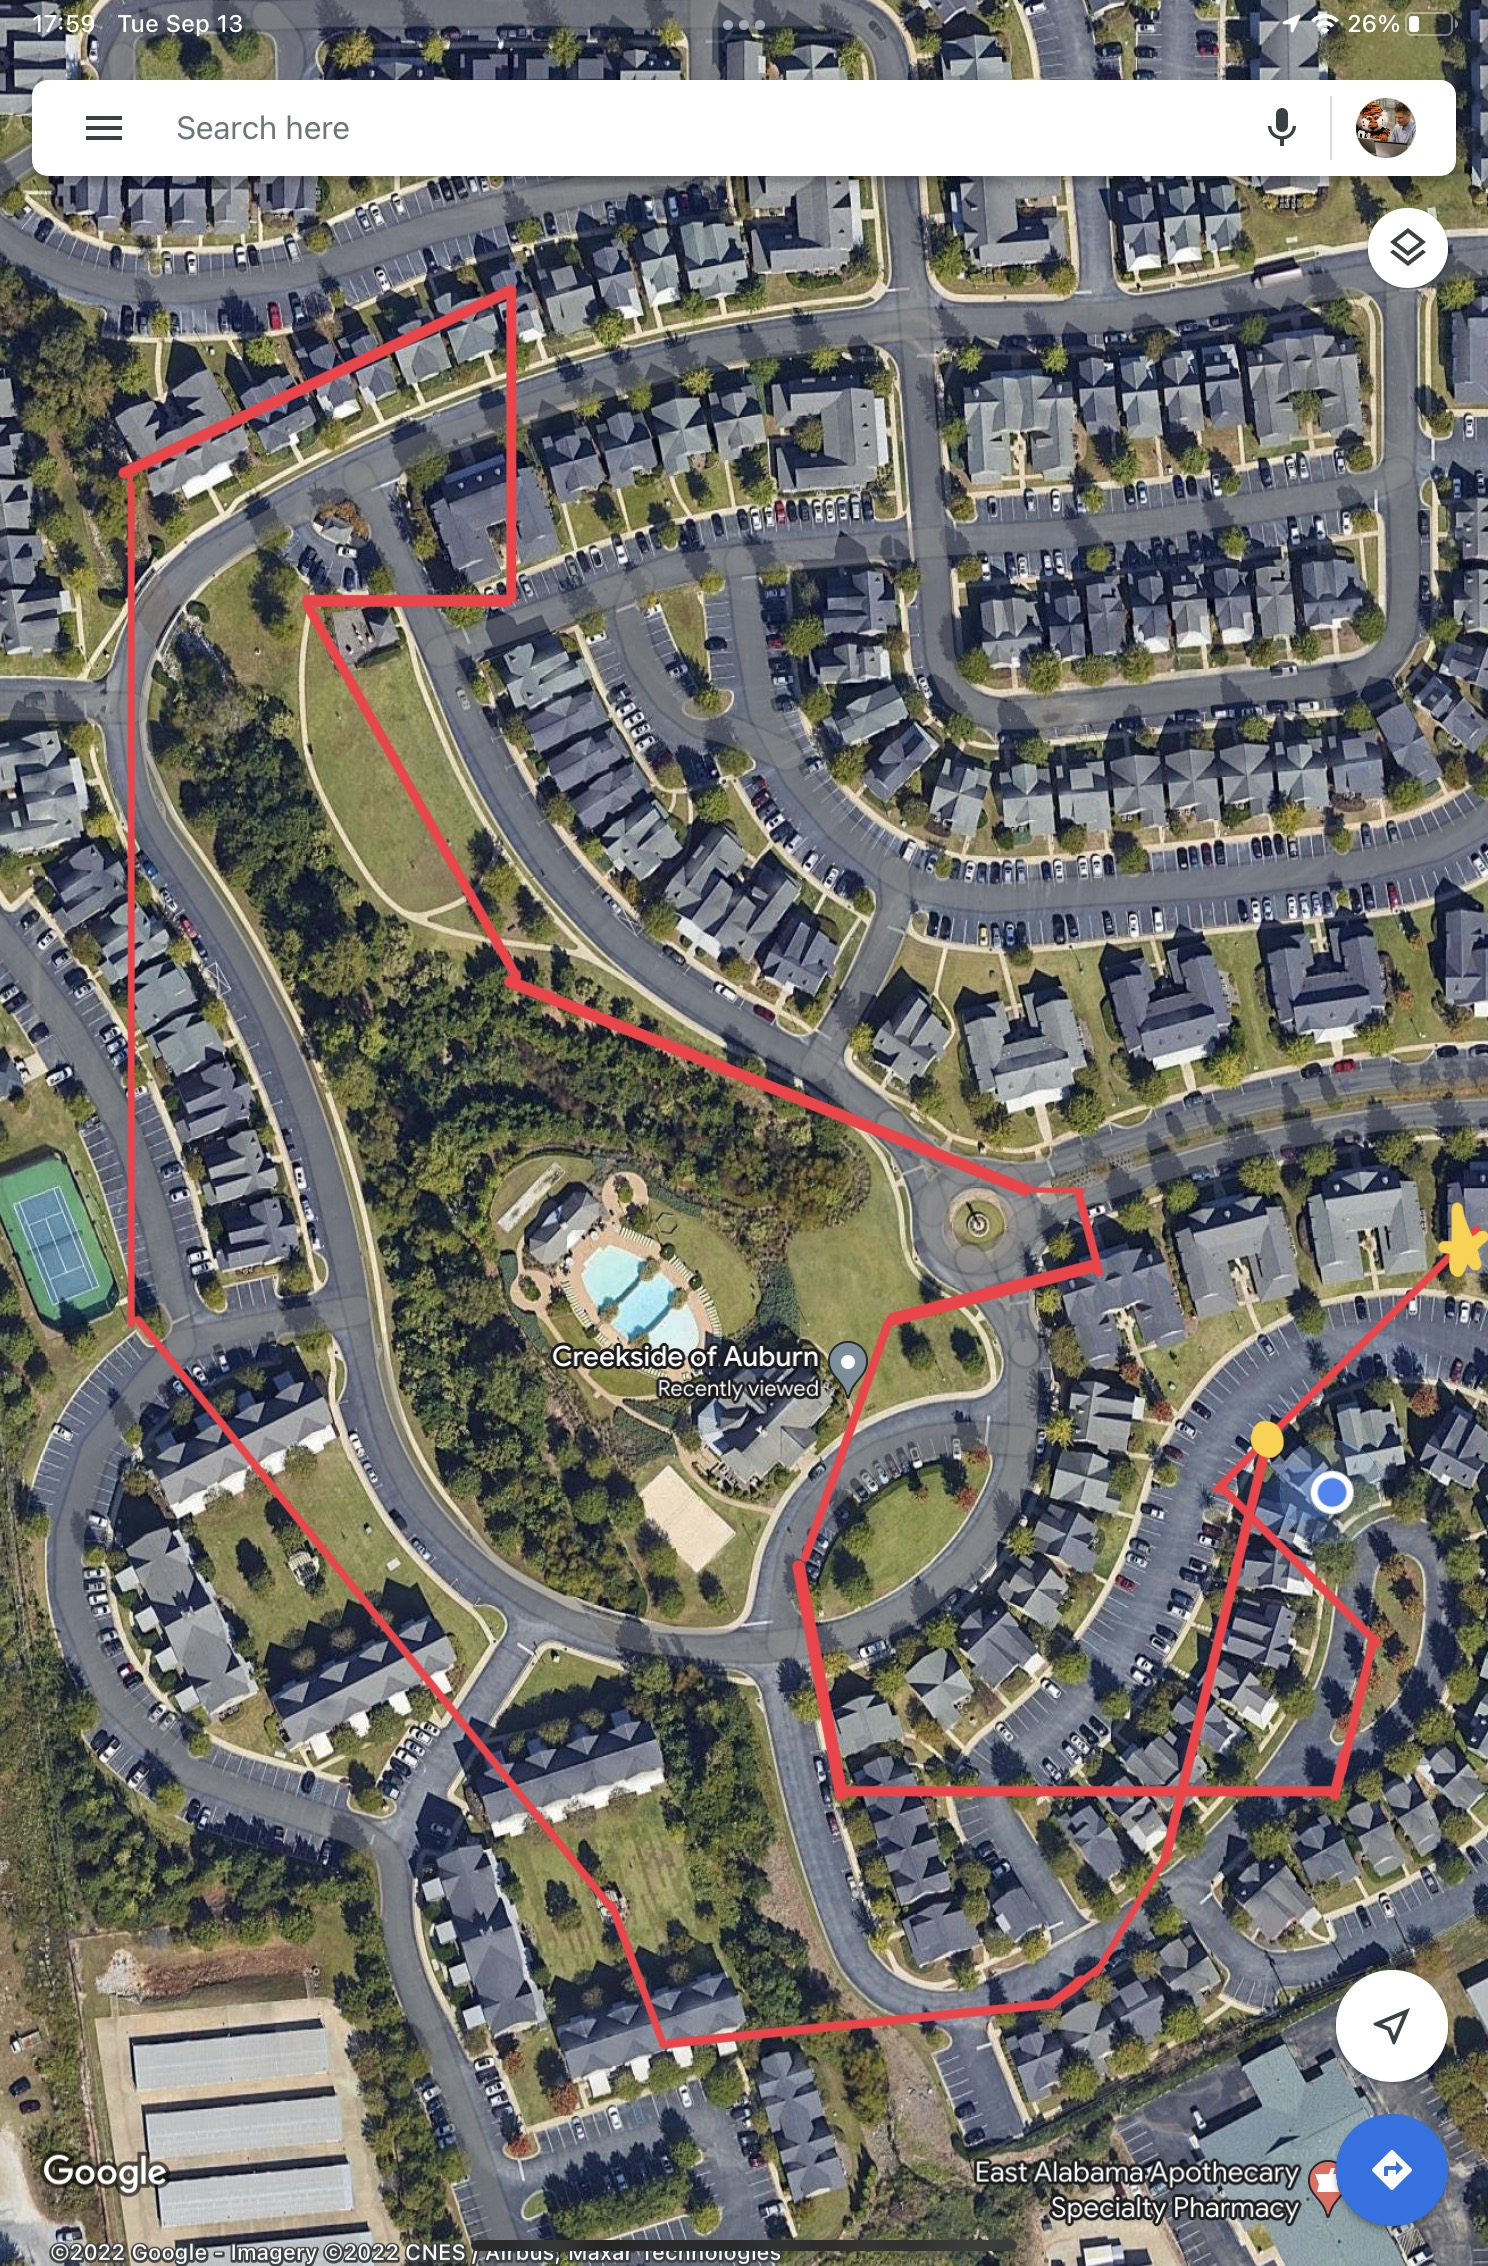
\includegraphics[width=0.5\linewidth]{IMG_0039.JPEG}
            \caption{Estimated path using step and compass measurements (Table \ref{tbl:1})}
            \label{fig:gmap_steps}
        \end{figure}
    }
    \clearpage
    \question{Find a scholarly article describing a navigation system for a team of at least two ground
        vehicles. Describe the sensors used, states estimated, and estimator architecture. Give a
        brief description of the problem statement/motivation for the work. What results were
        presented (e.g. plots of positioning accuracy, raw sensor data, etc.)? Did the authors
        successfully convey the methodology?}

    \solution{%
        In "Corridors-based naviation for automated vehicles convoy in off-road enviroments", the authors (Godoy J., et al.) present a motion-planning architecture based on the wake generation of the leading vehicle to optimally estimate a navigable trajectory. Godoy employs this methodology becuase markings found on highways and roads are either hard to detect using optical sensors, or just do not exist at all when travelling off-road. A handful of sensors colloborate to estimate the trajectory. These include:
        \begin{itemize}
            \item Radar
            \item Camera
            \item LiDAR
            \item IMU
            \item GNSS receivers
        \end{itemize}
        A localization algorithm uses the sensors above to feed into a perception algorithm. The outputs are then communicated to each following vehicle to where the guidance module takes over to feed the determined trajectory. They estimate the vehicles' position in the global frame, as well as the velocity and orientation of each vehicle with respect to the body frame. They also track the distance between each vehicle and try to maintain less than 50 meters between each vehicle, although some experiments showed the convoy separate by at least 60 meters. The authors display several plots over the course of the paper including plots on waypoint generation, average convoy speed, post-processed trajectories, and error over time with regard to leader-follower difference in speed, north position, and east position.

        I think the authors accurately conveyed their approach. They provide a theoretical algorithm and overview of their off-road grid planning trajectory system and then provide data from field tests with references to the steps inline with the algorithm block diagram.

    }
    \clearpage
    \question{In class, we developed the basic (elementary) rotation matrix
        \begin{equation*}
            C_{z,\theta} =
            \begin{bmatrix}
                cos(\theta) & -sin(\theta) & 0 \\
                sin(\theta) & cos(\theta)  & 0 \\
                0           & 0            & 1 \\
            \end{bmatrix}
        \end{equation*}
        that describe the orientation of a coordinate frame rotated away from another coordinate frame by an angle $\theta$ about the $y$-axis.}
    \begin{parts}
        \part{Derive the basic (elementary) rotation matrix $C_{y,\theta}$ that describes the orientation of a coordinate frame rotated away from another coordinate frame by an angle $\theta$ about the $y$-axis.}

        \solution{%
            \begin{figure}[!h]
                \centering
                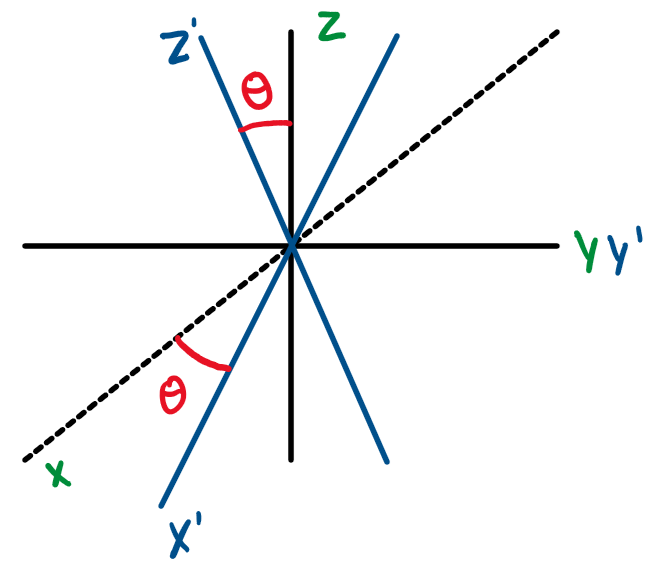
\includegraphics[width=0.5\linewidth]{Q3a.png}
                \caption{Standard 3-dimensional axis with an applied rotation, $\theta$, about the $y$-axis.}
                \label{fig:1}
            \end{figure}

            Using figure \ref{fig:1}, a $3 \times 3$ matrix comprised of dot products from each combination of unit vectors between the two frames and the rotation, $\theta$ will give us $C_{y,\theta}$.
            \begin{equation}
                \begin{split}
                    C_{y,\theta} & =
                    \begin{bmatrix}
                        x'x_1 & y'x_1 & z'x_1 \\
                        x'y_1 & y'y_1 & z'y_1 \\
                        x'z_1 & y'z_1 & z'z_1 \\
                    \end{bmatrix}\\
                    C_{y,\theta} & =
                    \begin{bmatrix}
                        cos(\theta)  & 0 & sin(\theta) \\
                        0            & 1 & 0           \\
                        -sin(\theta) & 0 & cos(\theta) \\
                    \end{bmatrix}\\
                \end{split}
                \label{eq:1}
            \end{equation}
        }
    \end{parts}
    \clearpage
    \question{For each of the matrices below, determine which are valid rotation matrices.  Justify
        your answer based upon expected properties.}

    \solution{%
        We can validate each rotation matrix by verifying that each matrix respects the orthonormality of rotation matrices.

        Orthonormality states that a matrix has indices orthogonal and normal to each other. We can check for orthonormality by using MATLAB command $>>det$ and the multiplication of the matrix with its transpose.
    }
    \begin{parts}
        \part{
            \begin{equation*}
                c^a_b =
                \begin{bmatrix}
                    0  & 0 & 1 \\
                    0  & 1 & 0 \\
                    -1 & 0 & 0 \\
                \end{bmatrix}
            \end{equation*}

            \solution{%
                \begin{equation}
                    \begin{split}
                        >>\mathbf{det}(c^a_b) = 1 \quad&\quad c^a_b \,(c^a_b)^{\mathbf{T}} =
                        \begin{bmatrix}
                            1 & 0 & 0 \\
                            0 & 1 & 0 \\
                            0 & 0 & 1 \\
                        \end{bmatrix} \\
                    \end{split}
                    \label{eq:2}
                \end{equation}
                Because the determinant of this matrix is 1 and the product of the matrix with it's transpose is the identity matrix, we can conclude that this is an actual rotation matrix.
            }
        }
        \part{
            \begin{equation*}
                c^b_c =
                \begin{bmatrix}
                    1 & 0 & -1 \\
                    0 & 1 & 0  \\
                    0 & 0 & 0  \\
                \end{bmatrix}
            \end{equation*}

            \solution{%
                \begin{equation}
                    \begin{split}
                        >>\mathbf{det}(c^b_c) = 0 \quad&\quad c^b_c \,(c^b_c)^{\mathbf{T}} =
                        \begin{bmatrix}
                            2 & 0 & 0 \\
                            0 & 1 & 0 \\
                            0 & 0 & 0 \\
                        \end{bmatrix} \\
                    \end{split}
                    \label{eq:3}
                \end{equation}
                This matrix is not a true rotation matrix as it is not orthogonal in it's components and also it's product with the matrix's transpose does not equal an identity matrix.
            }
        }
        \clearpage
        \part{
            \begin{equation*}
                c^c_d =
                \begin{bmatrix}
                    1 & 0           & 0 \\
                    0 & \frac{1}{2} & 0 \\
                    0 & 0           & 2 \\
                \end{bmatrix}
            \end{equation*}

            \solution{%
                \begin{equation}
                    \begin{split}
                        >>\mathbf{det}(c^c_d) = 1 \quad&\quad c^c_d \,(c^c_d)^{\mathbf{T}} =
                        \begin{bmatrix}
                            1 & 0    & 0 \\
                            0 & 0.25 & 0 \\
                            0 & 0    & 4 \\
                        \end{bmatrix} \\
                    \end{split}
                    \label{eq:4}
                \end{equation}
                While we do see that the rotation matrix is normal, it does not reflect an identity matrix after multiplying the transpose of itself. Because of this, we can say that this is not a true rotation matrix.
            }
        }
        \part{
            \begin{equation*}
                c^d_e =
                \begin{bmatrix}
                    0.4330  & -0.7718 & 0.4656 \\
                    0.7500  & 0.5950  & 0.2888 \\
                    -0.5000 & 0.2241  & 0.8365 \\
                \end{bmatrix}
            \end{equation*}

            \solution{%
                \begin{equation}
                    \begin{split}
                        >>\mathbf{det}(c^d_e) & = 0.99992\\
                        c^d_e \,(c^d_e)^{\mathbf{T}} & =
                        \begin{bmatrix}
                            0.99995             & -5.72\times 10^{-6} & 1.402\times 10^{-6} \\
                            -5.72\times 10^{-6} & 0.99993             & -7.93\times 10^{-5} \\
                            1.402\times 10^{-6} & -7.93\times 10^{-5} & 0.99995             \\
                        \end{bmatrix} \\
                    \end{split}
                    \label{eq:6}
                \end{equation}
                This rotation is tricky as MATLAB computes almost near perfect values to satisfy the orthonormal properties of a rotation matrix. However, solving this problem by hand gives us both orthogonality and an identity matrix, so we can conclude that this is a proper rotation matrix.
            }
            \part{
                \begin{equation*}
                    c^e_f =
                    \begin{bmatrix}
                        0.5000  & -0.1464 & 0.8536  \\
                        0.5000  & -0.8536 & -0.1464 \\
                        -0.7071 & 0.5000  & 0.5000  \\
                    \end{bmatrix}
                \end{equation*}

                \solution{%
                    \begin{equation}
                        \begin{split}
                            >>\mathbf{det}(c^e_f) = -0.45717 \quad&\quad c^e_f \,(c^e_f)^{\mathbf{T}} =
                            \begin{bmatrix}
                                1.0001  & 0.25     & 0.00005    \\
                                0.25    & 1.0001   & 0\-0.85355 \\
                                0.00005 & -0.85355 & 0.99995    \\
                            \end{bmatrix} \\
                        \end{split}
                        \label{eq:5}
                    \end{equation}
                    Here we see that this matrix is not a real rotation matrix as there is no orthogonality and no identity matrix produced from multiplying the matrix with it's transpose.
                }
            }
        }
    \end{parts}
    \clearpage
    \question{Consider the rotation matrix
        \begin{equation*}
            C^0_1 =
            \begin{bmatrix}
                0  & -\frac{\sqrt{3}}{2} & -\frac{1}{2}       \\
                0  & -\frac{1}{2}        & \frac{\sqrt{3}}{2} \\
                -1 & 0                   & 0                  \\
            \end{bmatrix}
        \end{equation*}}
    \begin{parts}
        \part{Sketch frames $0$ and $1$ with their origins co-located.}

        \solution{%
            \begin{figure}[!h]
                \centering
                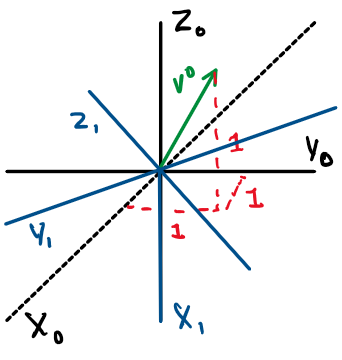
\includegraphics[width=0.5\linewidth]{Q5a.png}
                \caption{Sketch of both frames sharing a common origin.}
                \label{fig:2}
            \end{figure}
        }
        \part{Given a vector $\mathbf{v}^0 = \left[\;1 \quad 1 \quad 1\;\right]^T$ coordinated in frame $0$, re-coordinatize the vector such that it is described in frame 1.}

        \solution{%
            In order for us to transform $\mathbf{v}^0$ to frame 1, we can use the transformation matrix provided to us and multiply it by the original vector in frame 0.

            \begin{equation}
                \begin{split}
                    \mathbf{v}^1 & = \mathbf{C}^1_0 \mathbf{v}^0\\
                    \mathbf{v}^1 & =
                    \begin{bmatrix}
                        0  & -\frac{\sqrt{3}}{2} & -\frac{1}{2}       \\
                        0  & -\frac{1}{2}        & \frac{\sqrt{3}}{2} \\
                        -1 & 0                   & 0                  \\
                    \end{bmatrix}
                    \begin{bmatrix}
                        1 \\
                        1 \\
                        1 \\
                    \end{bmatrix}\\
                    \mathbf{v}^1 & =
                    \begin{bmatrix}
                        -1.3660 \\
                        0.3660  \\
                        -1.000  \\
                    \end{bmatrix}\\
                \end{split}
                \label{}
            \end{equation}
        }
    \end{parts}

    \question{For each pair of coordinate frames, find the rotation matrix $C^a_b$ that describes their relative orientation.}
    \begin{parts}
        \part{
            \solution{
                We can find the required rotation matrix $C^a_b$ by first rotating about the $Z$-axis by 90 degrees and then rotating by the intermediate $X$-axis by 180 degrees.
                \begin{figure*}[!h]
                    \centering
                    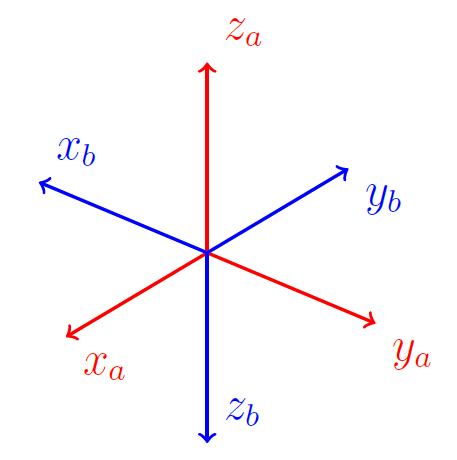
\includegraphics[width=0.25\linewidth]{Q6a.png}
                \end{figure*}

                This gives us a rotation sequence of
                \begin{equation}
                    C^a_b = \left(R_{z,90}\,R_{x,180}\right)^{\mathbf{T}}
                \end{equation}

                Using a custom MATLAB function (appended) we can easily find $C^a_b$ (Equation \ref{eq:9}).
                \begin{equation}
                    \begin{split}
                        C^a_b & =
                        \begin{bmatrix}
                            0  & -1 & 0  \\
                            -1 & 0  & 0  \\
                            0  & 0  & -1 \\
                        \end{bmatrix}^{\mathbf{T}}
                    \end{split}
                    \label{eq:9}
                \end{equation}
            }
        }
        \clearpage
        \part{
            \solution{
                We can find the required rotation matrix $C^a_b$ by first rotating about the $Y$-axis by 45 degrees and then rotating by the intermediate $X$-axis by 90 degrees.
                \begin{figure*}[!h]
                    \centering
                    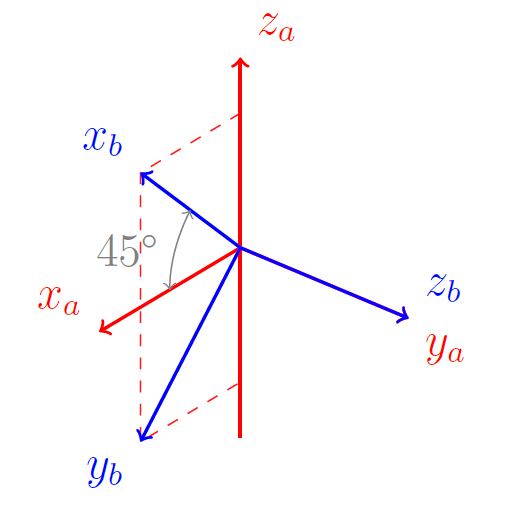
\includegraphics[width=0.25\linewidth]{Q6b.png}
                \end{figure*}

                This gives us a rotation sequence of
                \begin{equation}
                    C^a_b = \left(R_{Y,-45}\,R_{X,-90}\right)^{\mathbf{T}}
                \end{equation}

                Using a custom MATLAB function (appended) we can easily find $C^a_b$ (Equation \ref{eq:10}).
                \begin{equation}
                    \begin{split}
                        C^a_b & =
                        \begin{bmatrix}
                            \frac{\sqrt{2}}{2} & \frac{\sqrt{2}}{2}  & 0 \\
                                               &                     &   \\
                            0                  & 0                   & 1 \\
                                               &                     &   \\
                            \frac{\sqrt{2}}{2} & -\frac{\sqrt{2}}{2} & 0 \\
                        \end{bmatrix}^{\mathbf{T}}
                    \end{split}
                    \label{eq:10}
                \end{equation}
            }
        }
    \end{parts}
    \clearpage
    \question{Coordinate frame $\{1\}$ is obtained from frame $\{0\}$ by the following sequence of rotations:
        \begin{itemize}
            \item[i.]{$-90^o$ about the fixed $z$-axis}
            \item[ii.]{$90^o$ about the current $y$-axis}
            \item[iii.]{$-90^o$ about the fixed $x$-axis}
        \end{itemize}
        Find the resulting rotation matrix $C^0_1$ and sketch frames $\{0\}$ and $\{1\}$ relative to each other.
    }

    \solution{%
        From class, we know that relative rotations append to the current rotation and that fixed rotations prepend the current rotation, we can formulate the rotation $C^1_0$ to be
        \begin{equation*}
            C^1_0 = \left(R_{x,-90}R_{z,-90}R_{y,90}\right)^{\mathbf{T}}.
        \end{equation*}
        Then, using the same custom MATLAB function as used in question \ref{question@6}\ref{part@6@1}, we can calculate $C^0_1$.
        \begin{equation}
            \begin{split}
                C^0_1 & =
                \begin{bmatrix}
                    0 & -1 & 0 \\
                    1 & 0  & 0 \\
                    0 & 0  & 1 \\
                \end{bmatrix}\\
            \end{split}
            \label{eq:12}
        \end{equation}
        \begin{figure}[!h]
            \centering
            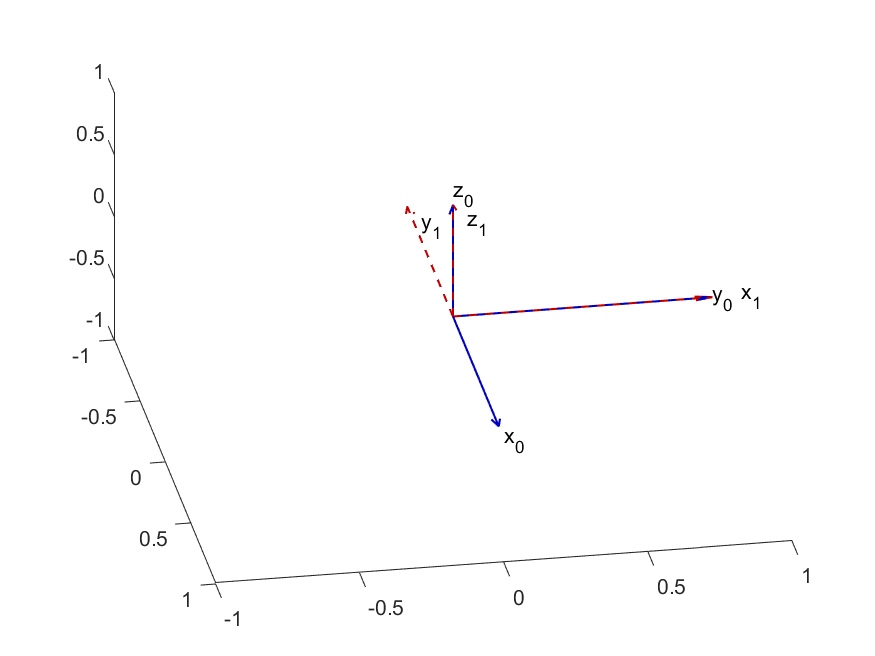
\includegraphics[width=0.75\linewidth]{Q7.png}
            \caption{Frame 0 rotated into frame 1 using a $R_{2\,3\,1}$ rotation matrix.}
            \label{fig:5}
        \end{figure}
    }
    \clearpage
    \question{Given the roll-pitch-yaw angles ($\phi$, $\theta$, $\psi$) = ($120^o$, $45^o$, $-120^o$), find the rotation matrix that describes the same orientation. Assume the $ZYX$ series of rotations. Verify that you have constructed the correct rotation matrix by backing out the angles.}

    \solution{%
    For a fixed rotation set of roll-pitch-yaw angles, we can find the rotation matrix by doing a fixed rotation sequence in 3 steps. This reflects that $C_0^1 = R_{\phi,120}\,R_{\theta,45}\,R_{\psi,-120}$. Multiplying these matrices together gives us
    \begin{equation*}
        C_0^1 =
        \begin{bmatrix}
            -0.35355 & 0.61237  & 0.70711  \\
            0.12683  & 0.78033  & -0.61237 \\
            -0.92678 & -0.12683 & -0.35355 \\
        \end{bmatrix}
    \end{equation*}

    To verify that this is correct we can back-solve for the Euler angles using the following equations (Equation \ref{eq:13}).
    \begin{equation}
        \begin{split}
            \phi & = tan^{-1}\left(\frac{-C_{23}}{C_{33}}\right) \\
            \theta & = tan^{-1}\left(\frac{C_{13}}{\sqrt{C_{23}^2 + C_{33}^2}}\right) \\
            \psi & = tan^{-1}\left(\frac{-C_{12}}{C_{11}}\right)\\
        \end{split}
        \label{eq:13}
    \end{equation}
    From equation \ref{eq:13}, we get
    \[\phi = -60^o \]
    \[\theta = 45^o \]
    \[\psi = 60^o \]
    and upon comparing our given rotation angles to these calculated ones, we are convinced that these angles are the same by understanding that angles can be noted in a positive rotation from $0^o$ to $180^o$.
    }
    \clearpage
    \question{(Required for 6790 only) Consider the threee coordinate frames $\{\alpha\}$, $\{\beta\}$, and $\{\gamma\}$ shown in the diagram below. Following the notation introduced in the class, find the following Cartesian position vectors (denoted by $\vec{r}$\;) and rotation matrices (denoted by $C$).
        \begin{figure*}[!h]
            \centering
            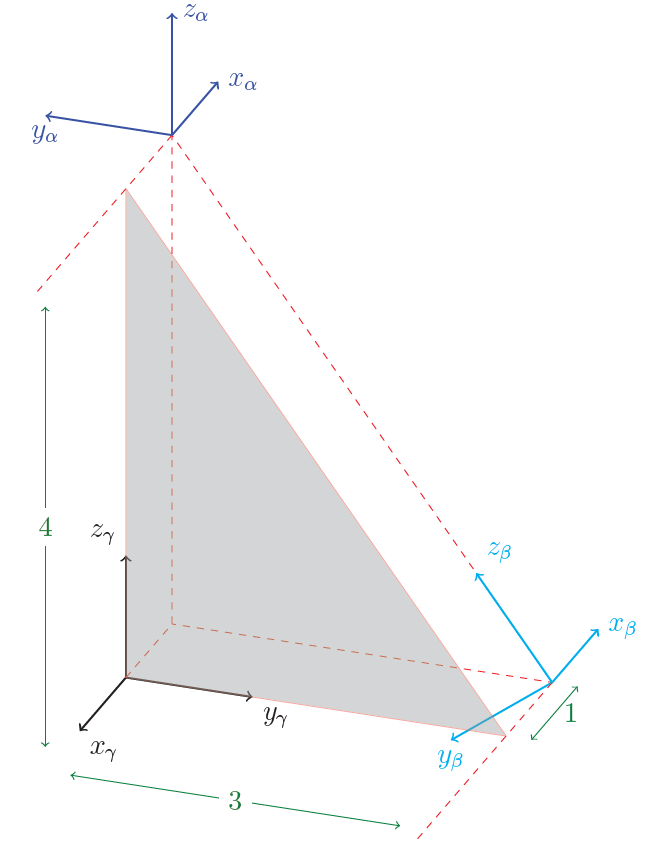
\includegraphics[width=0.85\linewidth]{Q9.png}
        \end{figure*}
        \clearpage
        \begin{parts}
            \part{$\vec{r}^{\,\gamma}_{\gamma\alpha}$}

            \solution{%
                We can find $\vec{r}^{\,\gamma}_{\gamma\alpha}$ by writing the vector components from $\gamma$ to $\alpha$ in the $\gamma$ frame.
                \begin{equation}
                    \begin{split}
                        \vec{r}^{\,\gamma}_{\gamma\alpha} & =
                        \begin{bmatrix}
                            \gamma_x - \alpha_x \\
                            \gamma_y - \alpha_y \\
                            \gamma_z - \alpha_z \\
                        \end{bmatrix}\\
                        \vec{r}^{\,\gamma}_{\gamma\alpha} & =
                        \begin{bmatrix}
                            0 - 1    \\
                            0 - 0    \\
                            0 - (-4) \\
                        \end{bmatrix}\\
                        \vec{r}^{\,\gamma}_{\gamma\alpha} & =
                        \begin{bmatrix}
                            -1 \\
                            0  \\
                            4  \\
                        \end{bmatrix}\\
                    \end{split}
                    \label{}
                \end{equation}
            }
            \part{$\vec{r}^{\,\gamma}_{\gamma\beta}$}

            \solution{%
                We can find $\vec{r}^{\,\gamma}_{\gamma\beta}$ by writing the vector components from $\gamma$ to $\beta$ in the $\gamma$ frame.
                \begin{equation}
                    \begin{split}
                        \vec{r}^{\,\gamma}_{\gamma\beta} & =
                        \begin{bmatrix}
                            \gamma_x - \beta_x \\
                            \gamma_y - \beta_y \\
                            \gamma_z - \beta_z \\
                        \end{bmatrix}\\
                        \vec{r}^{\,\gamma}_{\gamma\beta} & =
                        \begin{bmatrix}
                            0 - 1    \\
                            0 - (-3) \\
                            0 - 0    \\
                        \end{bmatrix}\\
                        \vec{r}^{\,\gamma}_{\gamma\beta} & =
                        \begin{bmatrix}
                            -1 \\
                            3  \\
                            0  \\
                        \end{bmatrix}\\
                    \end{split}
                    \label{}
                \end{equation}}
            \part{$\vec{r}^{\,\alpha}_{\gamma\alpha}$}

            \solution{%
                We can find $\vec{r}^{\,\alpha}_{\gamma\alpha}$ by writing the vector components from $\gamma$ to $\alpha$ in the $\alpha$ frame.
                \begin{equation}
                    \begin{split}
                        \vec{r}^{\,\alpha}_{\gamma\alpha} & =
                        \begin{bmatrix}
                            \gamma_x - \alpha_x \\
                            \gamma_y - \alpha_y \\
                            \gamma_z - \alpha_z \\
                        \end{bmatrix}\\
                        \vec{r}^{\,\alpha}_{\gamma\alpha} & =
                        \begin{bmatrix}
                            0 - (-1) \\
                            0 - 0    \\
                            0 - 4    \\
                        \end{bmatrix}\\
                        \vec{r}^{\,\alpha}_{\gamma\alpha} & =
                        \begin{bmatrix}
                            1  \\
                            0  \\
                            -4 \\
                        \end{bmatrix}\\
                    \end{split}
                    \label{}
                \end{equation}}
            \part{$\vec{r}^{\,\beta}_{\gamma\beta}$}

            \solution{%
                We can find $\vec{r}^{\,\beta}_{\gamma\beta}$ by writing the vector components from $\gamma$ to $\beta$ in the $\beta$ frame.
                \begin{equation}
                    \begin{split}
                        \vec{r}^{\,\beta}_{\gamma\beta} & =
                        \begin{bmatrix}
                            \gamma_x - \beta_x \\
                            \gamma_y - \beta_y \\
                            \gamma_z - \beta_z \\
                        \end{bmatrix}\\
                        \vec{r}^{\,\beta}_{\gamma\beta} & =
                        \begin{bmatrix}
                            0 - (-1) \\
                            0 - 3    \\
                            0 - 0    \\
                        \end{bmatrix}\\
                        \vec{r}^{\,\beta}_{\gamma\beta} & =
                        \begin{bmatrix}
                            1  \\
                            -3 \\
                            0  \\
                        \end{bmatrix}\\
                    \end{split}
                    \label{}
                \end{equation}}
            \part{${C}^{\gamma}_{\alpha}$}

            \solution{%
                Finding the direction cosine matrix from $\alpha$ to $\gamma$ is a simple $R_{Z,180}$ rotation.
                \begin{equation}
                    \begin{split}
                        {C}^{\gamma}_{\alpha} & =
                        \begin{bmatrix}
                            -1 & 0  & 0 \\
                            0  & -1 & 0 \\
                            0  & 0  & 1 \\
                        \end{bmatrix}
                    \end{split}
                    \label{}
                \end{equation}
            }
            \part{${C}^{\gamma}_{\beta}$}

            \solution{%
            Finding the direction cosine matrix from $\beta$ to $\gamma$ is a simple $R_{X,45}R_{Z,180}$ rotation.
            \begin{equation}
                \begin{split}
                    {C}^{\beta}_{\alpha} & =
                    \begin{bmatrix}
                        -1 & 0                   & 0                   \\
                           &                     &                     \\
                        0  & -\frac{\sqrt{2}}{2} & -\frac{\sqrt{2}}{2} \\
                           &                     &                     \\
                        0  & -\frac{\sqrt{2}}{2} & \frac{\sqrt{2}}{2}  \\
                    \end{bmatrix}
                \end{split}
                \label{}
            \end{equation}
            }
            \part{${C}^{\alpha}_{\beta}$}

            \solution{%
                Finding the direction cosine matrix from $\beta$ to $\alpha$ is a simple $R_{X,45}$ rotation.
                \begin{equation}
                    \begin{split}
                        {C}^{\alpha}_{\beta} & =
                        \begin{bmatrix}
                            1 & 0                  & 0                   \\
                              &                    &                     \\
                            0 & \frac{\sqrt{2}}{2} & -\frac{\sqrt{2}}{2} \\
                              &                    &                     \\
                            0 & \frac{\sqrt{2}}{2} & \frac{\sqrt{2}}{2}  \\
                        \end{bmatrix}
                    \end{split}
                    \label{}
                \end{equation}
            }
        \end{parts}
    }

\end{questions}
\end{document}